\documentclass{report}
\title{An Introductory Course in Computational Neuroscience---Paul Miller (Notes)}
\date{Started 14 Dec 2024}
\author{Malcolm}
\usepackage{amsmath} %import math
\usepackage{mathtools} %more math
\usepackage{amssymb} %for QED symbol
\usepackage{amsthm} %
\usepackage{bm} %bolding without changing font
\usepackage{graphicx} %import imaging
\graphicspath{{./images/}} %set imaging path
\newcommand*{\vertbar}{\rule[-1ex]{0.5pt}{2.5ex}} %matrix
\newcommand*{\horzbar}{\rule[.5ex]{2.5ex}{0.5pt}} %matrix
\begin{document}
\maketitle
\tableofcontents
\newpage

\section{xLIF}
\subsection{Modelling the Leaky membrane potential}
\textbf{Nernst Potential}\\
The \textit{Nernst potential} $E_A$ of an ion $A$ of charge $z_A$ with intracellular concentration $[A_{\text{in}}]$ and extracellular concentration $[A_{\text{out}}]$ is given by
\begin{equation*}
E_A=\frac{k_BT}{z_Aq_e}\ln\left(\frac{[A_{\text{out}}]}{[A_{\text{in}}]}\right)
\end{equation*}
where $T$ is the temperature in Kelvin, $k_B$ the Boltzmann constant $(1.39\times10^{-23}JK^{-1})$ (which converts units of temperature to units of thermal energy). $q_e$ is the fundamental electronic charge
$(1.60\times10^{-19}C)$.\\
\vspace{1mm}\\
\textbf{Model}\\
Considering this representation of a neuron's membrane:
\begin{figure}[h]
\begin{center}
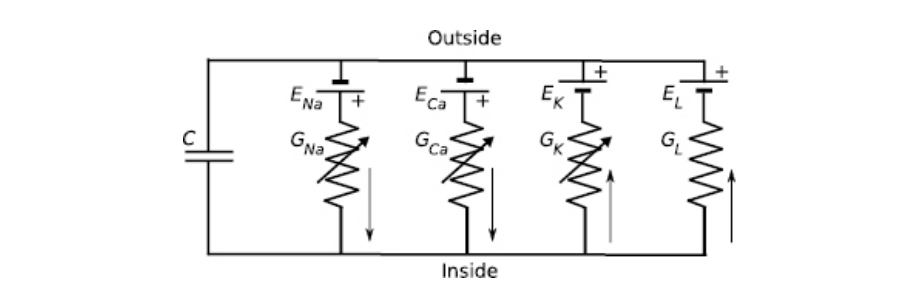
\includegraphics[width=10cm]{1}\\
\end{center}
If all channels with variable conductance are closed, then the current will only flow through the leak channels (subscript $L$) until the cell membrane is at the leak
potential $E_L$. The current through a channel is given by
\begin{equation*}
I_t=G_t(V_m-E_t)
\end{equation*}
Where $G_t$ represents conductance and $E_t$ the nernst potential; $t$ represents the type of channel.
\end{figure}\\
(next page)
\newpage
\noindent\textbf{Equilibrium}\\
When the cell is at equilibrium the different currents balance each other out and sum to zero:
\begin{equation*}
I_m=\sum_tI_t=\sum_tG_t(V_m-E_t)=0
\end{equation*}
In the context of this current model this can be rewritten as
\begin{equation*}
G_{Na}(V_m-E_{Na})+G_{Ca}(V_m-E_{Ca})+G_{K}(V_m-E_{K})
+G_{L}(V_m-E_{L})
\end{equation*}
Solving for $V_m$ we can see that the \textit{resting membrane potential}---where no net current flows, is the weighted average of the individual Nernst potentials:
\begin{equation*}
V_m=\frac{G_{Na}E_{Na}+G_{Ca}E_{Ca}+G_{K}E_{K}+G_{L}E_{L}}{G_{Na}+G_{Ca}+G_{K}+G_{L}}
\end{equation*}
The derivation of the resting membrane potential is typically more complicated.\\
\vspace{1mm}\\
\textbf{Leaky membrane potential}\\
Here we consider the passive properties of the cell, where the variable conductance of all channels are fixed. With this the we treat the circuit as having
a single `leak' conductance and potential.\\
\vspace{1mm}\\
The membrane potential is generated by the charge stored on the membrane; it depends on both the stored charge and the membrane's capacitance $C_m$ via the equation
\begin{equation*}
Q=C_mV_m
\end{equation*}
The current is defined as positive when it flows \textit{out} of the cell; with that we have
\begin{equation*}
\frac{dQ}{dt}=-I_m=-G_L(V_m-E_L)
\end{equation*}
Fixing the capacitance we obtain the dynamics of the resting membrane potential as
\begin{equation*}
C_m\frac{dV_m}{dt}=G_L(E_L-V_m)
\end{equation*}
This is a linear first order ODE. 
\newpage

\subsection{Solution for Leaky ODE}
We had the dynamics of the resting membrane potential as
\begin{equation*}
C_m\frac{dV_m}{dt}=G_L(E_L-V_m)
\end{equation*}
Expressing in standard form and solving by integrating factor:
\begin{align*}
\frac{dV_m}{dt}+\frac{G_L}{C_m}V_m&=\frac{G_L}{C_m}E_L\\
V_m&=\frac{1}{\exp\left(\frac{G_L}{C_m}t\right)}\left(\int\exp\left(\frac{G_L}{C_m}t\right)\cdot\frac{G_L}{C_m}E_L\,dt+c\right)
\end{align*}
To simplify we define the \textit{time constant} $\tau_m=C_m/G_L$:
\begin{align*}
V_m&=\frac{1}{\exp\left(\frac{t}{\tau_m}\right)}\left(\int\exp\left(\frac{1}{\tau_m}t\right)\cdot\frac{1}{\tau_m}E_L\,dt+c\right)\\
&=\exp\left(-\frac{t}{\tau_m}\right)\left(\exp\left(\frac{t}{\tau_m}\right)E_L+A\right)\\
&=E_L+\exp\left(-\frac{t}{\tau_m}\right)\cdot A
\end{align*}
At initial condition $V_m(0)$:
\begin{equation*}
V_m(0)=E_L+A\implies A=V_m(0)-E_L
\end{equation*}
With that we have the solution
\begin{equation*}
V_m=E_L+(V_m(0)-E_L)\exp\left(-\frac{t}{\tau_m}\right)
\end{equation*}
(next page)
\newpage
\noindent\textbf{Illustrated}\\
See that the equation tends to $E_L$, and that $\tau_m$ dictates how fast this decay occurs (thus the name). Illustrated here using code from \texttt{leakymembrane.py}:
\begin{figure}[h]
\begin{equation*}
V_m=E_L+(V_m(0)-E_L)\exp\left(-\frac{t}{\tau_m}\right)
\end{equation*}
\begin{center}
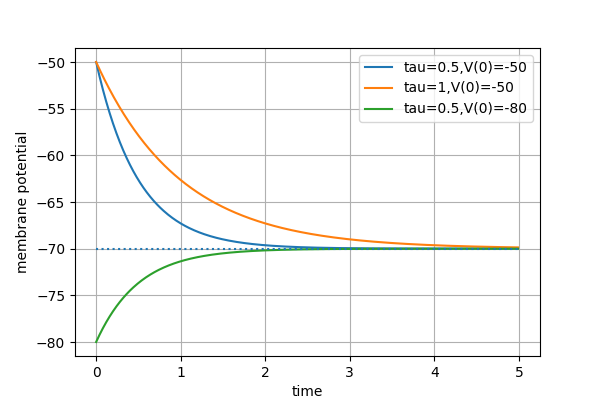
\includegraphics[width=10cm]{2}\\
\end{center}
\end{figure}
\newpage

\subsection{Leaky-Integrate-and-Fire}
The LIF introduces a framework on which we can build more realistic models of neurons. It is essentially the intial model
for the leaky membrane with an additional term $I_\text{app}$ modelling an applied current. The spike is modelled by the membrane potential being reset 
to a low (hyperpolarised) value $V_\text{reset}$
after the potential reaches some threshold $V_{th}$ (threshold potential):
\begin{equation*}
C_m\frac{dV_m}{dt}=G_L(E_L-V_m)+I_\text{app};\text{if $V_m>V_{th}$ then $V_m\mapsto V_\text{reset}$}
\end{equation*}
Notice that an actual `spike' shape hasn't been modelled, and would have to be put in by hand before $V_m$ is reset; spike times are recorded at the time when
the membrane potential crosses the threshold.\\
\vspace{1mm}\\
The following was simulated using code from \texttt{LIFfunc.py}:
\begin{figure}[h]
\begin{center}
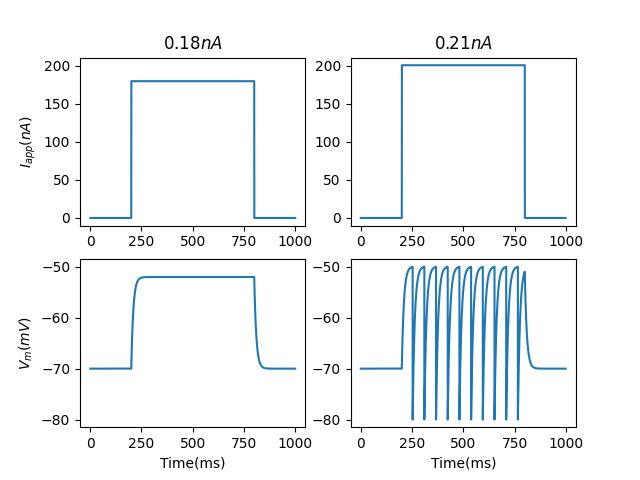
\includegraphics[width=9cm]{3}\\
\end{center}
\textbf{Threshold current}\\
See that there is an insufficient level for $I_{\text{app}}$ where no `firing' occurs (the membrane potential does not reach threshold and the model does not spike).
Setting $dV_m/dt=0$ allows us to obtain the \textit{steady state} membrane potential as
\begin{equation*}
V^{ss}_m=E_L+I_{\text{app}}/G_L
\end{equation*}
If the steady state is below threshold then the model does not fire. By setting
$V^{ss}_m=V_{th}$ we can obtain the \textit{threshold current} $I_{th}$---the minimum applied
current required to elicit firing:
\begin{equation*}
I_{th}=G_L(V_{th}-E_L)
\end{equation*}
\end{figure}
\newpage

\subsection{Firing rate-Current (F-I) curve of the LIF model}
For the LIF (and fixed applied current), we can come up with a closed-form way of determining the time for the neuron's 
membrane potential to increase from its reset value to the threshold.\\
\vspace{1mm}\\
\textbf{Solution for LIF model with constant $I_{\text{app}}$}\\
Ignoring the hard reset part of the LIF (this doesn't matter since we are trying to find time between a period where the model doesn't reset), we have
\begin{equation*}
C_m\frac{dV_m}{dt}=G_L(E_L-V_m)+I_\text{app}
\end{equation*}
When the applied current is fixed this equation can be solved:
\begin{equation*}
V_m(t)=V^{ss}_m+\left(V_m(0)-V^{ss}_m\right)\exp\left(-\frac{t}{\tau_m}\right)
\end{equation*}
where $V^{ss}_m$ denotes the steady state membrane potential.\\
\vspace{1mm}\\
\textbf{Interspike Interval (ISI)}\\
We want the time $T$ when the next spike is produced, so we have $V_m(T)=V_{th}$ and solve for it. We also set the initial condition to $V_{\text{reset}}$ since we
want the time between reset and threshold:
\begin{equation*}
V_{th}=V_m(T)=V^{ss}_m+\left(V_{\text{reset}}-V^{ss}_m\right)\exp\left(-\frac{T}{\tau_m}\right)
\end{equation*}
Rearranging:
\begin{equation*}
\exp\left(-\frac{T}{\tau}\right)=\frac{V_{th}-V^{ss}_m}{V_\text{reset}-V^{ss}_m}
=\frac{V^{ss}_m-V_{th}}{V^{ss}_m-V_\text{reset}}
\end{equation*}
See that the term on the right must be positive and less than 1 for a solution to exist with $T>0$; since $0<e^{-x}<1$ for all real $x>0$.\\
\vspace{1mm}\\
This reflects the fact that we can only calculate the time between spikes if $V^{ss}_m>V_{th}$ for spiking to occur in the first place.
(If $V_{\text{reset}}<V^{ss}_m<V_{th}$ the right side would be negative; if $V^{ss}_m<V_{\text{reset}}<V_{th}$ it would be greater than 1.)\\
\vspace{1mm}\\
Solving for $T$ gives us the time from one spike to the next---the \textit{interspike interval} (ISI):
\begin{equation*}
\text{ISI}=T=-\tau_m\ln\left(\frac{V^{ss}_m-V_{th}}{V^{ss}_m-V_\text{reset}}\right)
=\tau_m\ln\left(\frac{V^{ss}_m-V_{th}}{V^{ss}_m-V_\text{reset}}\right)
\end{equation*}
(next page)
\newpage
\noindent\textbf{Firing rate}\\
The firing rate is the inverse of the ISI:
\begin{equation*}
f(I_{app})=\frac{1}{\text{ISI}}=\frac{1}{\tau_m\ln\left(\frac{V^{ss}_m-V_{th}}{V^{ss}_m-V_\text{reset}}\right)}=
\frac{1}{\tau_m\ln\left(\frac{E_L+I_{\text{app}}/G_L-V_{th}}{E_L+I_{\text{app}}/G_L-V_\text{reset}}\right)}
\end{equation*}
This is a rare case where we have a closed form solution for the firing rate curve. 
\newpage

\subsection{Solution for LIF with fixed applied current and no reset}
Ignoring the hard reset part of the LIF and fixing $I_{\text{app}}$, we have
\begin{equation*}
C_m\frac{dV_m}{dt}=G_L(E_L-V_m)+I_\text{app}
\end{equation*}
This can be solved. Where $\tau=C_m/G_L$:
\begin{equation*}
\frac{dV_m}{dt}=\frac{G_L}{C_m}(E_L-V_m)+\frac{I_\text{app}}{C_m}
\end{equation*}
In standard form:
\begin{equation*}
\frac{dV_m}{dt}+\frac{1}{\tau}V_m=\frac{1}{\tau}E_L+\frac{I_\text{app}}{C_m}
\end{equation*}
Solving by integrating factor:
\begin{align*}
V_m(t)&=\frac{1}{\exp(t/\tau)}\left(\int\exp\left(\frac{t}{\tau}\right)\left(\frac{1}{\tau}E_L+\frac{I_\text{app}}{C_m}\right)\,dt+c\right)\\
&=\exp\left(-\frac{t}{\tau}\right)\left(\tau\exp\left(\frac{t}{\tau}\right)\left(\frac{1}{\tau}E_L+\frac{I_\text{app}}{C_m}\right)+A\right)\\
&=\exp\left(-\frac{t}{\tau}\right)\left(\exp\left(\frac{t}{\tau}\right)E_L+\exp\left(\frac{t}{\tau}\right)\tau\frac{I_\text{app}}{C_m}+A\right)\\
&=E_L+\frac{C_m}{G_L}\frac{I_\text{app}}{C_m}+A\exp\left(-\frac{t}{\tau}\right)\\
&=E_L+\frac{I_\text{app}}{G_L}+A\exp\left(-\frac{t}{\tau}\right)
\end{align*}
Initial condition:
\begin{align*}
V_m(0)&=E_L+\frac{I_\text{app}}{G_L}+A\\
A&=V_m(0)-\left(E_L+\frac{I_\text{app}}{G_L}\right)
\end{align*}
We have the solution
\begin{equation*}
V_m(t)=E_L+\frac{I_\text{app}}{G_L}+\left(V_m(0)-\left(E_L+\frac{I_\text{app}}{G_L}\right)\right)\exp\left(-\frac{t}{\tau}\right)
\end{equation*}
(next page)
\newpage
\noindent\textbf{In relation to steady state potential}\\
We had
\begin{equation*}
V_m(t)=E_L+\frac{I_\text{app}}{G_L}+\left(V_m(0)-\left(E_L+\frac{I_\text{app}}{G_L}\right)\right)\exp\left(-\frac{t}{\tau}\right)
\end{equation*}
Recall that setting $dV_m/dt=0$ in the LIF equation (again ignoring the hard reset) gave us the steady state membrane potential $V^{ss}_m$:
\begin{equation*}
V^{ss}_m=E_L+I_{\text{app}}/G_L
\end{equation*}
See that this can be slotted into our solution:
\begin{equation*}
V_m(t)=V^{ss}_m+\left(V_m(0)-V^{ss}_m\right)\exp\left(-\frac{t}{\tau}\right)
\end{equation*}
\newpage

\subsection{Simulated firing rate vs Calculated firing rate}
The following was plotted using code from \texttt{f-i\_curves.py}:
\begin{figure}[h]
\begin{center}
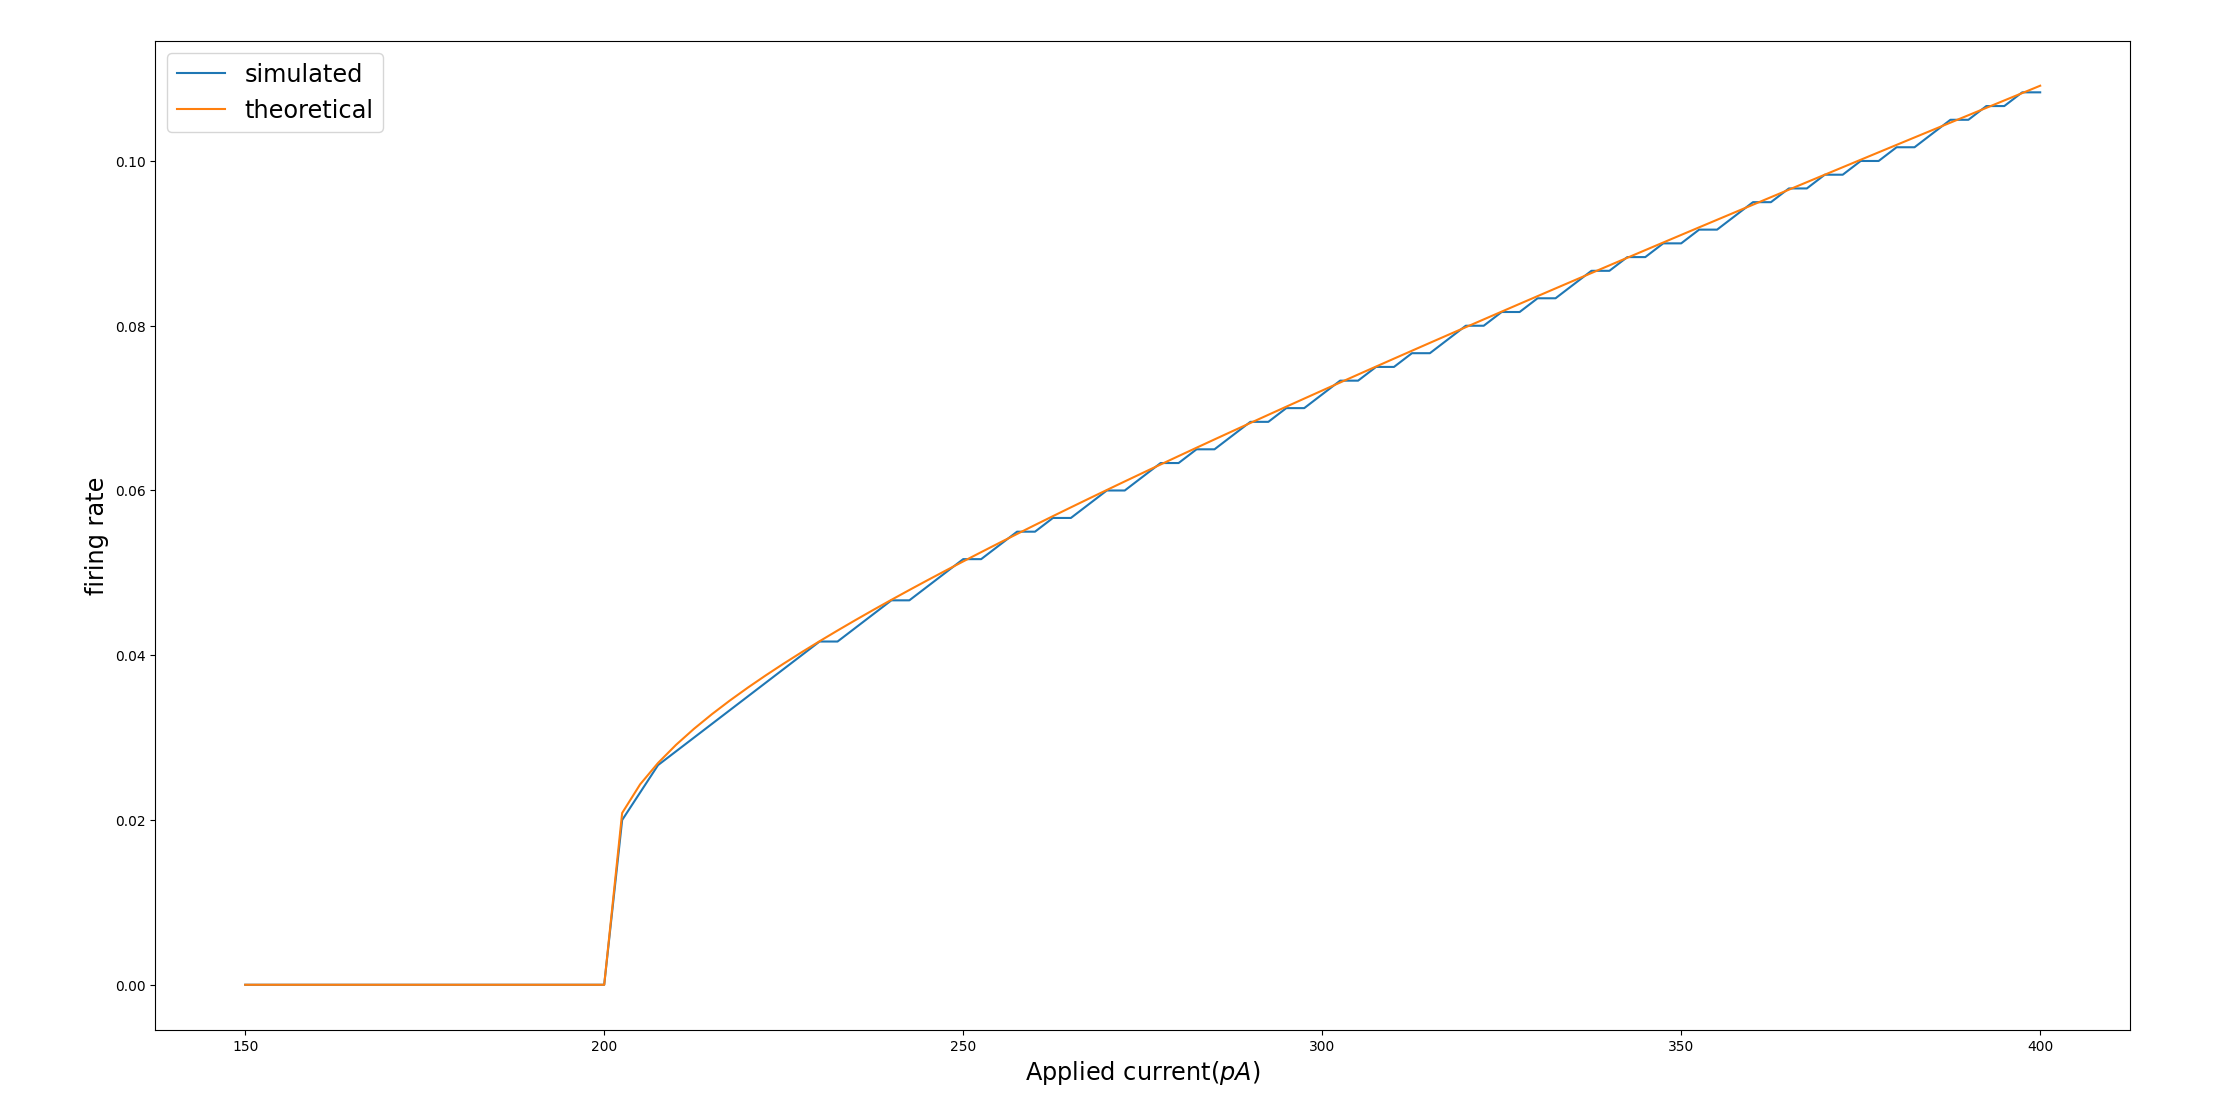
\includegraphics[width=10cm]{4}\\
\end{center}
LIF neurons were initialised with default parameters outlined in \texttt{LIFclass.py}. 
Applied currents ranging from 150 to 400$pA$ were applied; simulated firing rate was
calculated and compared to separately calculated theoretical firing rate values.
\end{figure}\\
The threshold current, if calculated from the default values for this simulation, is
200$pA$. See that this coincides with the simulation---spiking only starts after applied
current exceeds threshold current.
\newpage

\subsection{Euler-Mayamara method---LIF with noise}
Noise can be incorporated using a white noise process $w(t)$, defined as having zero mean.\\ 
\vspace{1mm}\\
\textbf{Definition}\\
Here we define noise as having variance equal to a delta function in time, so that
\begin{equation*}
\mathbb{E}[w(t)]=0\quad\text{and}\quad\mathbb{E}[w(t)w(t')]=\delta(t-t')
\end{equation*}
(the second equality holds since mean is zero)
The delta function is defined to be 0 unless $t=t'$; the idea here is that the value of $w(t)$ is uncorrelated with the value of $w(t')$ unless $t=t'$ 
(which would also mean that $w(t)=w(t')$).\\
\vspace{1mm}\\
\textbf{Simulating}\\
The delta-function has the property where its integral over all time is equal to one:
\begin{equation*}
\int^\infty_{-\infty}\delta(t-t')\,dt=1
\end{equation*}
it has units of inverse-time $(s^{-1})$; this means that the white noise function has units of the square-root of inverse time $(s^{-0.5})$ (this is important in
simulations---it indicates how to scale the term with each timestep). \\
\vspace{1mm}\\
When we update the variable (in this case using the forward euler method), 
the noise term is thus included as:
\begin{equation*}
x_{n+1}=x_n+f(x_n)\Delta t+\sigma\tilde{w}_n\sqrt{\Delta t}
\end{equation*}
Where $\tilde{w}_n$ is a random number selected from a distribution of 0 mean and unit variance (in order to satisfy the earlier definition---the noise at any given time point 
is not correlated with any other point, and has variance 1).
\begin{center}
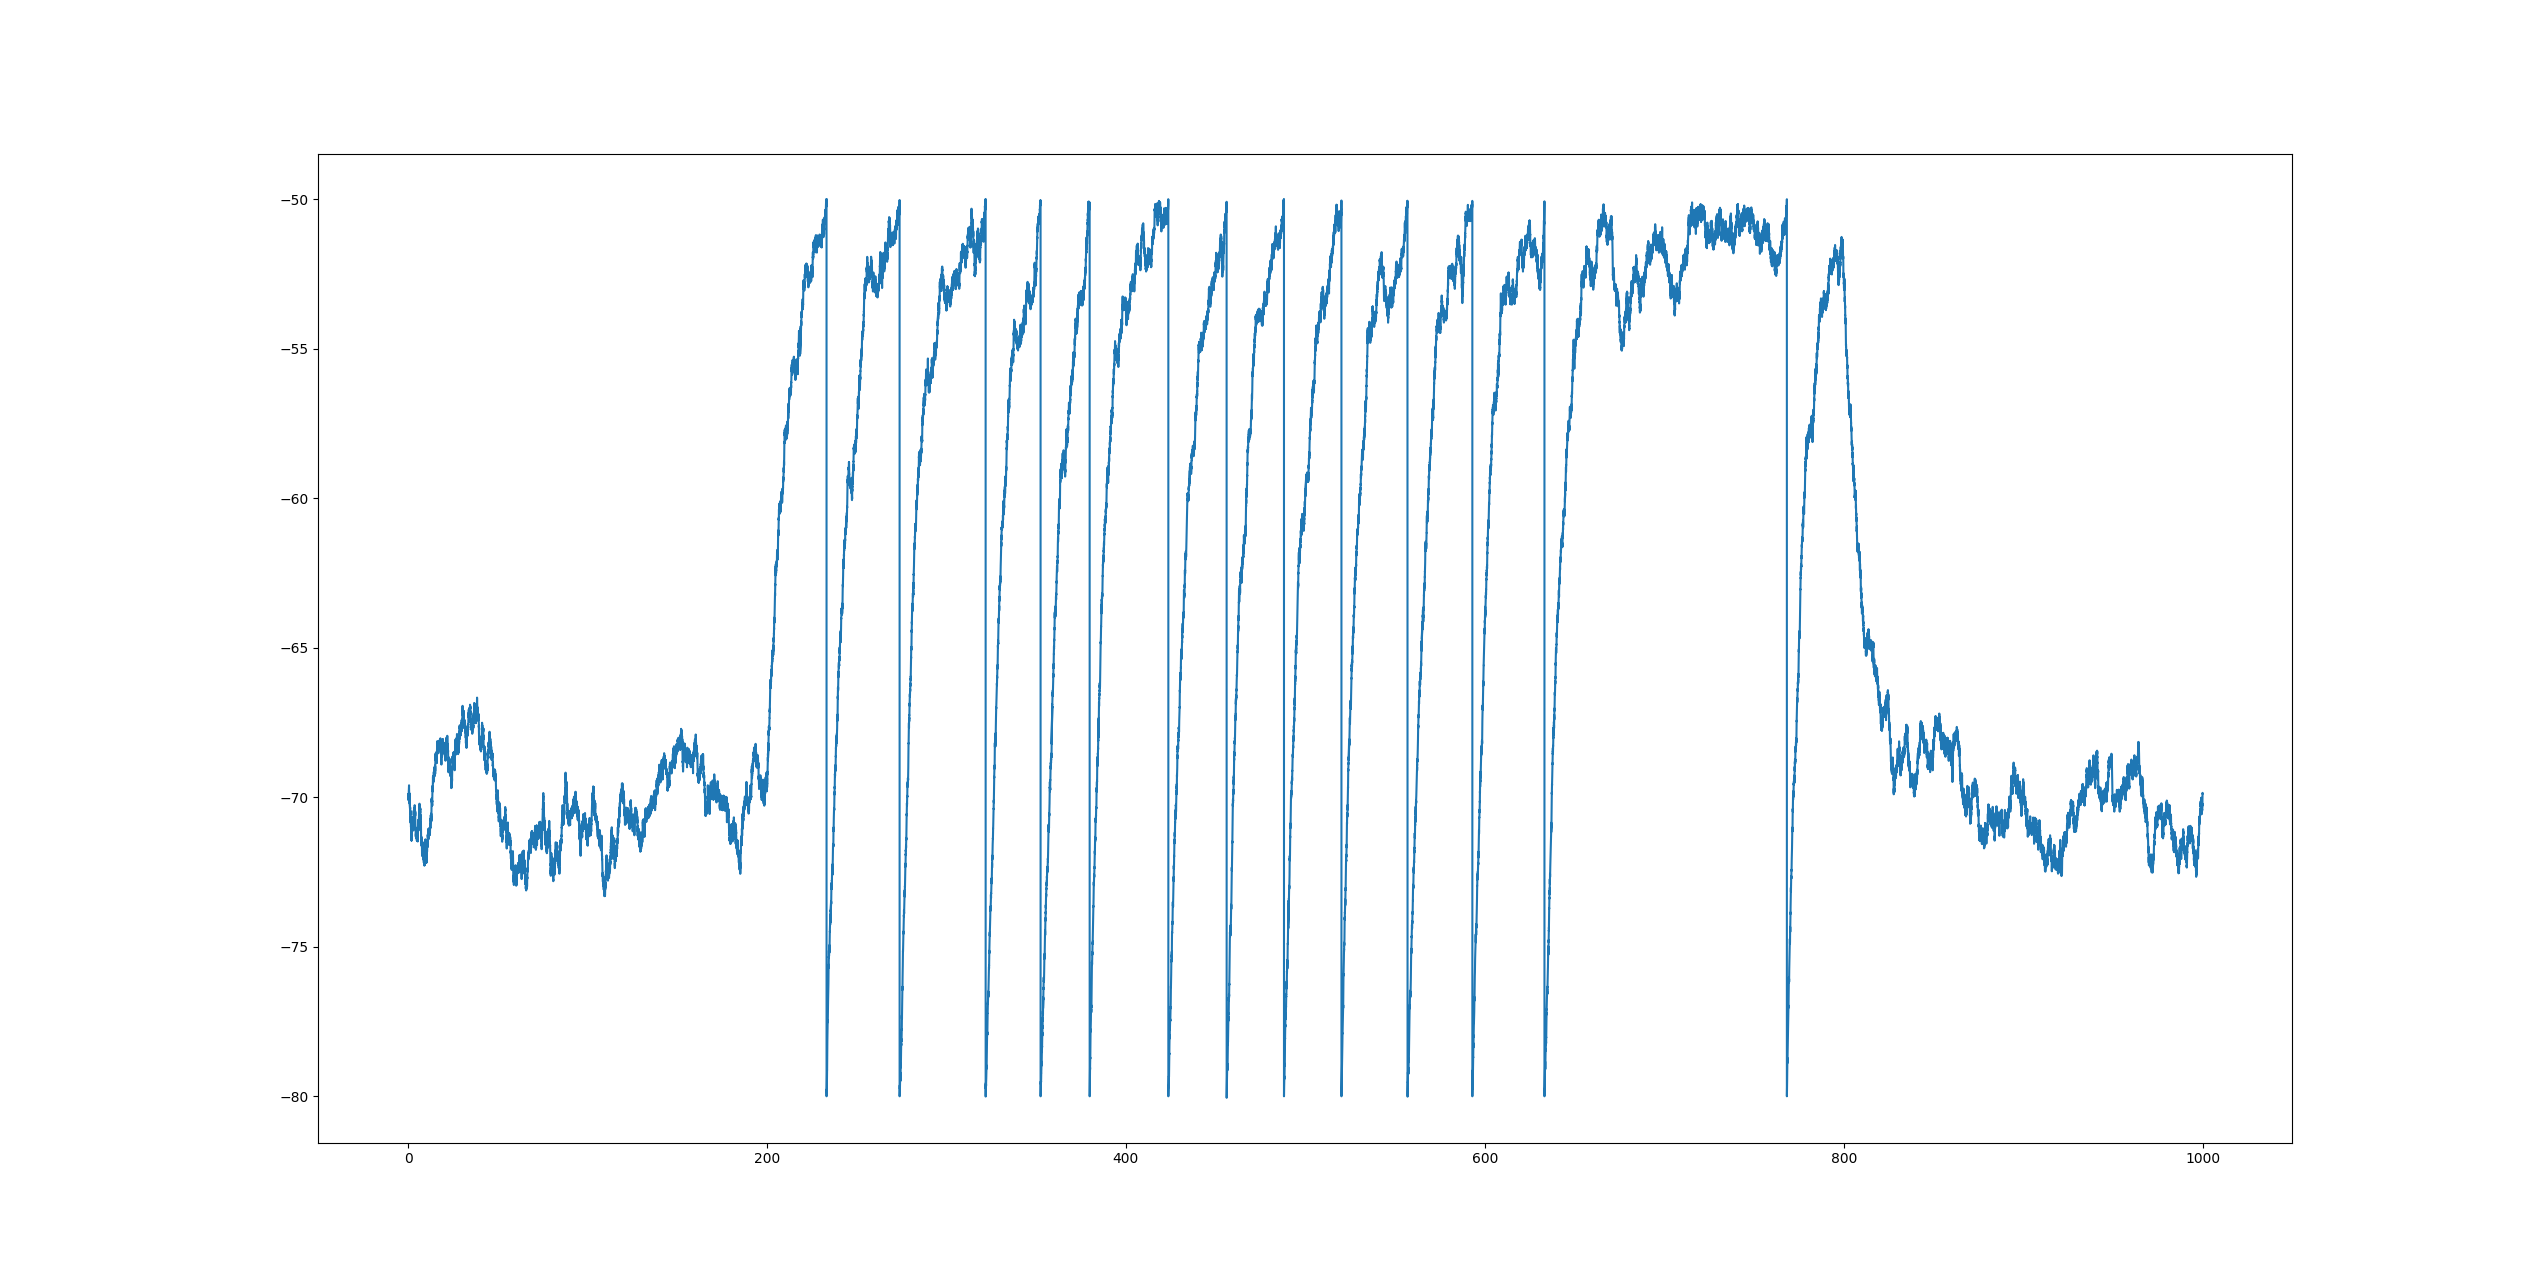
\includegraphics[width=10cm]{5}\\
\end{center}
Figure: Noise incorporated with $\sigma_I$ set to 0.5, see \texttt{LIFwithnoise.py}.
\newpage

\subsection{Models for the refractory period}
\textbf{Model 1: Forced Voltage Clamp}\\
Fix the voltage at its reset value folllowing a spike for the duration of the refractory period.\\
\vspace{1mm}\\
One disadvantage to this would be that the as the firing rate of the neuron increases, the neuron spends a greater proportion of its time in the refractory period 
(with the membrane potential at its low reset value). The mean membrane potential can decrease with increased input in such a model, unlike real neurons.\\
\vspace{1mm}\\
\textbf{Model 2: Refractory Conductance}\\
The refractory period can be mimicked by addition of a large conductance that produces a large outward (hyperpolarising) \textit{potassium current}. This refractory
conductance increases at the time of each spike and decays between spike times with a short time constant:
\begin{equation*}
\frac{dG_{\text{ref}}(t)}{dt}=-\frac{G_{\text{ref}}(t)}{\tau_{\text{ref}}}\quad\text{after spike }G_{\text{ref}}\mapsto G_{\text{ref}}+\Delta G
\end{equation*}
See that since we model this as an outward potassium current, it yields an additional term of
\begin{equation*}
G_{\text{ref}}[E_k-V_m(t)]
\end{equation*}
Where $E_k$ denotes the nernst potential for potassium ions. See that when $G_{\text{ref}}$ is much larger that the leak conductance this will essentially clamp the membrane
potential at $E_k$.\\
\vspace{1mm}\\
Also see that this means that the reset step of the LIF model can be omitted in simulations using this method, because the step increase in $G_{\text{ref}}$ will cause the 
desired drop in membrane potential.
Our final model looks like
\begin{equation*}
C_m\frac{dV_m}{dt}=G_L(E_L-V_m)+I_\text{app}+G_{\text{ref}}[E_k-V_m(t)]
\end{equation*}
Unlike the first method, in this method the time spent at the reset value depends on the strength of the other currents entering the neuron---the stronger the other inputs the more quickly they can overcome the decaying refractory current.
\newpage
\noindent\textbf{Model 3: Raised Threshold}\\
The




\end{document}
